\documentclass[12pt, french, latin.medieval, a4paper]{report}
% package de langues 
\usepackage[french]{babel}
\usepackage[utf8]{inputenc}
\usepackage[T1]{fontenc}

% package pour référence de liens sur pdf 
\usepackage[pdftex]{hyperref} % liens
\usepackage{lastpage} % numéro de page
\usepackage{caption}

% package de formes de document 
\usepackage[left=2.5cm,
              right=2.5cm,
              top=2.5cm,
              bottom=2.5cm
             ]{geometry}
% pour les tableaux 
\usepackage{array,multirow,makecell} 
\newcolumntype{R}[1]{>{\raggedleft\arraybackslash }b{#1}}
\newcolumntype{L}[1]{>{\raggedright\arraybackslash }b{#1}}
\newcolumntype{C}[1]{>{\centering\arraybackslash }b{#1}}

% package pour la page de couverture 
\usepackage{graphicx}
\usepackage[cyr]{aeguill}
\usepackage{fancyheadings}
\usepackage{amsmath}
\usepackage{amsfonts}
\usepackage{amssymb}
\usepackage{geometry}
\usepackage{eso-pic}
\usepackage{tikz}
\usetikzlibrary{calc}


% nouvelle commande pour la forme 
%\fancyhf[OFC]{\thepage / \pageref{LastPage}}
\rfoot{\thepage / \pageref{LastPage}}
%\setcounter{tocdepth}{3}

% pakages de couleurs du document
\usepackage{color}
\usepackage{xcolor}


% package pour la chimie
\usepackage[version=4]{mhchem}


% package pour la visualisation du code
\usepackage{listings}
\definecolor{darkWhite}{rgb}{0.94,0.94,0.94}
 
\lstset{
  aboveskip=3mm,
  belowskip=-2mm,
  backgroundcolor=\color{darkWhite},
  basicstyle=\footnotesize,
  breakatwhitespace=false,
  breaklines=true,
  captionpos=b,
  commentstyle=\color{red},
  deletekeywords={...},
  escapeinside={\%*}{*)},
  extendedchars=true,
  framexleftmargin=16pt,
  framextopmargin=3pt,
  framexbottommargin=6pt,
  frame=tb,
  keepspaces=true,
  keywordstyle=\color{blue},
  language=python,
  literate=
  {²}{{\textsuperscript{2}}}1
  {⁴}{{\textsuperscript{4}}}1
  {⁶}{{\textsuperscript{6}}}1
  {⁸}{{\textsuperscript{8}}}1
  {€}{{\euro{}}}1
  {é}{{\'e}}1
  {è}{{\`{e}}}1
  {ê}{{\^{e}}}1
  {ë}{{\¨{e}}}1
  {É}{{\'{E}}}1
  {Ê}{{\^{E}}}1
  {û}{{\^{u}}}1
  {ù}{{\`{u}}}1
  {â}{{\^{a}}}1
  {à}{{\`{a}}}1
  {á}{{\'{a}}}1
  {ã}{{\~{a}}}1
  {Á}{{\'{A}}}1
  {Â}{{\^{A}}}1
  {Ã}{{\~{A}}}1
  {ç}{{\c{c}}}1
  {Ç}{{\c{C}}}1
  {õ}{{\~{o}}}1
  {ó}{{\'{o}}}1
  {ô}{{\^{o}}}1
  {Õ}{{\~{O}}}1
  {Ó}{{\'{O}}}1
  {Ô}{{\^{O}}}1
  {î}{{\^{i}}}1
  {Î}{{\^{I}}}1
  {í}{{\'{i}}}1
  {Í}{{\~{Í}}}1,
  morekeywords={*,...},
  numbers=left,
  numbersep=10pt,
  numberstyle=\tiny\color{black},
  rulecolor=\color{black},
  showspaces=false,
  showstringspaces=false,
  showtabs=false,
  stepnumber=1,
  stringstyle=\color{gray},
  tabsize=4,
  title=\lstname,
}

%package pour les algorithmes
\usepackage{algorithm}
\usepackage{algorithmic}
\usepackage{amsmath}

% package pour les tableaux
\usepackage{longtable}
\usepackage{booktabs}

% package pour les figures 
\usepackage{subcaption}

% package de reférencement
% \usepackage[backend=biber,safeinputenc, sorting=none]{biblatex}

% mettre la bibliographie dans la table de matières
%\usepackage[nottoc, notlof, notlot]{tocbibind}
\include{page_couverture.tex}


\author{MBE MBE MINDJANA LOIC HENRI}
\title{GNPS et MDByTE}

\begin{document}
    
    \pagecouverture
    {Combinaison GNPS et MADByTE}
    {}
    \tableofcontents
    \vspace{20cm}
    
    \section{Introduction}
        Pour réaliser l'identification des molécules du vivant par la déréplication de nos jours, on utilise deux outils, à savoir GNPS qui permet d'obtenir sur la base d'un ensemble de spectres tandem \textbf{MS/MS} (MS pour Mass Spectrometry) un réseau moléculaire et MADByTE permettant aussi le faire mais sur la base de spectres 2D-RMN (RMN pour Résonnance Magnétique Nucléaire) \textbf{HSQC} (Heteronuclear Single Quantum Coherence) et \text{TOCSY} (Total Correlation Spectroscopy). Toutefois malgré leur utilité qui n’est plus à démontrer, on n’arrive pas à exploiter complètement l’espace chimique des molécules avec ces outils séparément pour mieux identifier les molécules. C’est dans le but de mieux prendre en compte cet espace chimique que la question suivante s’offre à nous, \textbf{comment combiner l'utilisation des spectres MS/MS et HSQC-TOCSY, pour mieux réaliser la déréplication ?}. Dans les lignes qui suivent nous parlerons d'abord de la déréplication et de sa relation avec l’identification tel que nous l'avons perçu, ensuite des outils GNPS et MADByTE pour réaliser cette déréplication, et enfin de l’idée de combinaison que nous avons.

    \section{Identification et Déréplication}

        La déréplication est un processus qui permet d'identifier une molécule ou encore un ensemble de molécules dit "d’inconnu" par des méthodes de spectrométries, tel que la spectrométrie de masse, la spectroscopie au rayon UV, la spectroscopie par résonnance magnétique nucléaire, etc…. Elle conduit ainsi par implication à l’identification de molécules connues dans un ensemble de molécules incertaines. 

        Cette méthode d’identification s’appuyant sur les spectres des molécules (qui constituent un espace chimique), cherche à capturer des correspondances entre ces dernières qui s’observent des similarités mesurées entre elles. Ces correspondances permettent de lier ces molécules entre elles, qu’elles soient connues ou non en utilisant leurs spectres. Prenons le cas des molécules \textbf{surfacin C13[M+Na]}, \textbf{surfacin C14[M+Na]} et \textbf{surfacin C15[M+Na]}; sur la base de leurs spectres MS, on peut sans connaitre leurs structures moléculaires savoir qu’elles sont de la même famille comme on peut le voir sur la figure \ref{fig:spectresmssurfacin}.
        
        \begin{figure}
            \centering
            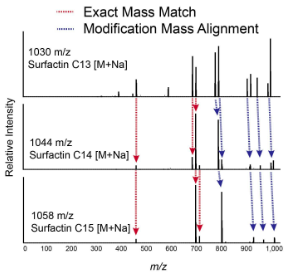
\includegraphics[]{Images/surfacins.png}
            \caption{Spectres MS de surfacin \cite{wang2016sharing}}
            \label{fig:spectresmssurfacin}
        \end{figure}

        Sur cette figure \ref{fig:spectresmssurfacin}, on peut remarquer qu’on a des pics en commun exacts (suivant la dimension masse sur charge), des pics en commun très peu déplacés (selon la dimension masse sur charge), des atténuations et accentuations (selon la dimension d'intensité relative), qui mettent en évidence le fait que les molécules sont très proches et donc de la même famille. Les déplacements faibles, atténuations et accentuations des pics traduisent les spécificités structurelles des molécules car permettent de les différentiées. De ces pics, ceux qu’on pourrait qualifiées de semblables constituent un bloc commun qu’on peut qualifier de pattern utile pour identifier leur famille.
        
        Cette méthode permet donc de retrouver une ou des molécules connues dans un ensemble de molécules, sur la base d’autres enregistrées, et ou d’identifier une ou des molécules inconnues dans un ensemble de molécules qui contient des molécules connues, tout ceci sans connaitre les structures moléculaires des molécules. Ainsi comment GNPS et MADByTE sont utilisés pour réaliser de la déréplication.



    \section{GNPS}
        L'outil GNPS (Global Natural Product Social Molecular Networking) est la résultante de l'article \cite{wang2016sharing}, qui attaquait la problématique de partage et d'extraction de connaissance d'une grande quantité de données spectrales MS/MS dans le but d'effectuer la déréplication. La raison de son développement vient du fait que la capture d’informations des spectres ne se faisait pas sur une grande quantité de spectres et n'utilisait pas des modèles d'interprétation efficace pour effectuer la déréplication plus facilement. Il utilise le modèle d’interprétation appelé réseau molécule pour mieux apprécier les différentes liaisons entre les spectres. Pour comprendre comment il fonctionne, nous devons savoir ce qu’est un spectre MS et un spectre MS/MS.

        \subsection{Spectres MS et MS/MS}
            Un spectre de masse MS est la donnée obtenue de la spectrométrie de masse d’un composé chimique ou d’une molécule, à haute ou à basse résolution. Elle permet d’avoir une signature spectrale d’un élément, dans le sens où elle est l’ensemble des couples d’intensités- masses sur charge des radicaux (qui sont les pics) obtenus après ionisation de l’élément en question. 
            
            Les spectres MS/MS eux sont obtenues après une double ionisation, c’est-à-dire que les radicaux obtenus en MS sont encore ionisés pour avoir une signature plus précise, d’où la raison d’utiliser un spectromètre de masse à haute résolution. Dans ce cas, comment GNPS utilise les spectres d’entrée pour arriver au réseau moléculaire dans le but réaliser la déréplication ?


        \subsection{Workflow de GNPS et déréplication}
            Pour construire un réseau moléculaire, GNPS utilise un ensemble de molécules connues dont les spectres sont contenus dans sa base publique. Cette base de spectres \ref{fig:basegnps} est nourrie en utilisant des spectres de librairies publiques tel que MassBank, ReSpect et par des résultats des expériences validées par des paires.

            \begin{figure}
                \centering
                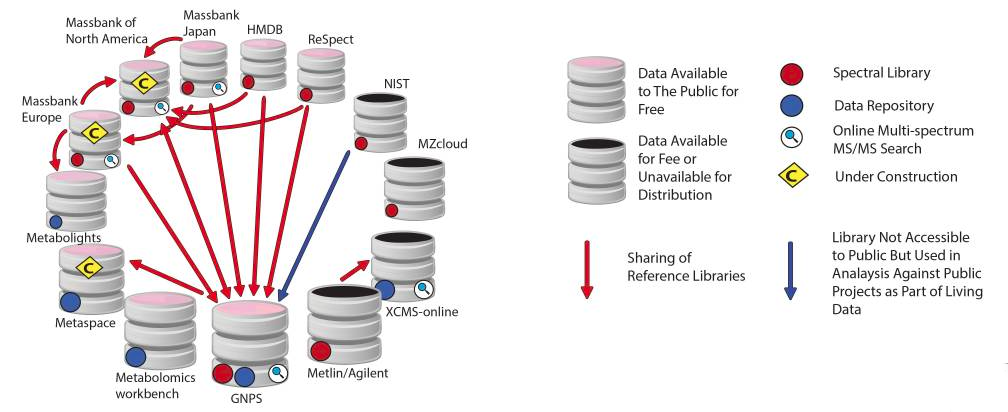
\includegraphics[width=\linewidth]{Images/GNPS10.png}
                \caption{Schéma de peuplement de la base GNPS \cite{wang2016sharing}}
                \label{fig:basegnps}
            \end{figure}

            GNPS utilise un workflow \ref{fig:gnps} ayant deux branches parallèles :
            \begin{enumerate}
                \item La recherche de spectres existants : permettant de retrouver les spectres d’entrée de molécules qui se trouvent déjà dans la base publique GNPS

                \item La construction du graphe de spectres : permettant de relier tous les spectres de molécules d’entrée qui sont similaire entre eux. L’ensemble de liaisons construites entre les spectres MS/MS permet d’avoir un graphe, où un nœud est un spectre de molécule et où une arête est une relation de similarité entre deux spectres
            \end{enumerate}

            \begin{figure}
                \centering
                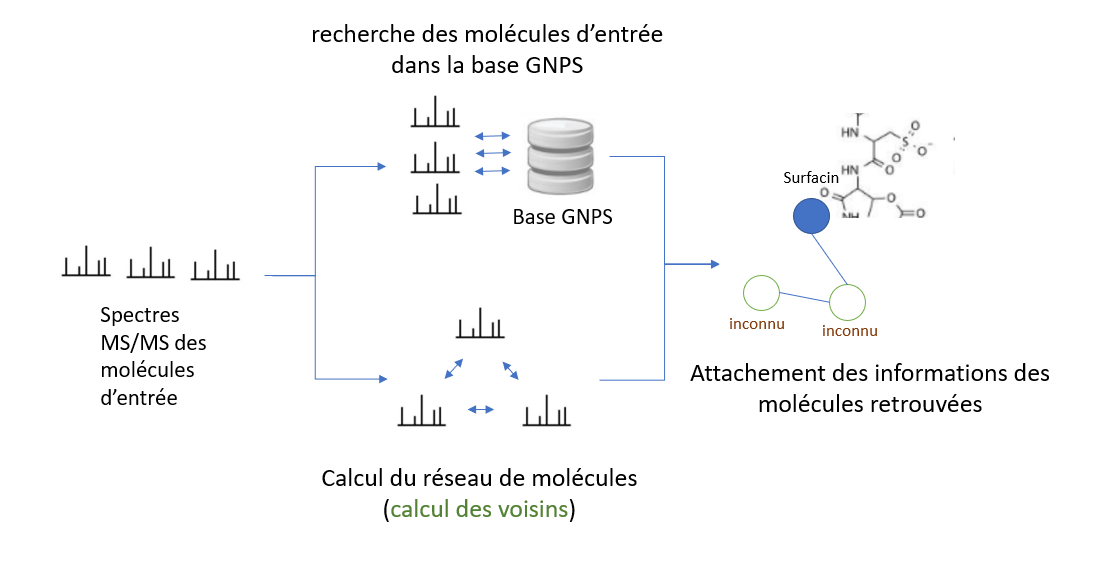
\includegraphics[width=\linewidth]{Images/gnps.png}
                \caption{Vue simplifiée du Workflow de GNPS}
                \label{fig:gnps}
            \end{figure}

            Après création du graphe et fouille des spectres dans la base publique GNPS, on ajoutera des métadonnées des spectres retrouvés dans la base (comme le nom de la molécule du spectre, la structure moléculaire encodé en SMILE ou en INCHI, …) sur leurs nœuds correspondants. Ceux qui ne seront pas retrouvés auront l’étiquette "inconnu", ce qui permet finalement d’avoir un graphe de spectres retrouvés (connus) et non retrouvés (inconnus) reliés par rapport aux liens de similarité entre eux. 

            Dans la figure du workflow détaillé \ref{fig:gnps_org}, on peut se rendre compte qu’afin de mesurer la similarité entre deux spectres "sp1" et un autre "sp2" on utilise une mesure de similarité, qui est le cosinus de similarité $cos (sp1, sp2)$ dont on a la formule \ref{form:cosinus}. On considère que deux spectres sont voisins, si leur cosinus de similarité est supérieur à un seuil de "ressemblance" (couramment égale \textbf{0.6}), et que deux spectres sont identiques si leur cosinus est plutôt supérieur à un seuil d’identification (couramment égale à \textbf{0.7}). Il faut noter que ces seuils doivent être donner par un expert pour obtenir des relations correctes, plus on aura des valeurs faibles, plus on cherchera à effectuer de l'exploration de relations.

            \begin{equation}
                \cos(sp1, sp2) = \frac{<sp1, sp2>}{||sp1||\times||sp2||}\ avec\ \cos(sp1, sp2) \in [-1, 1]
                \label{form:cosinus}
            \end{equation}
            
            \begin{figure}
                \centering
                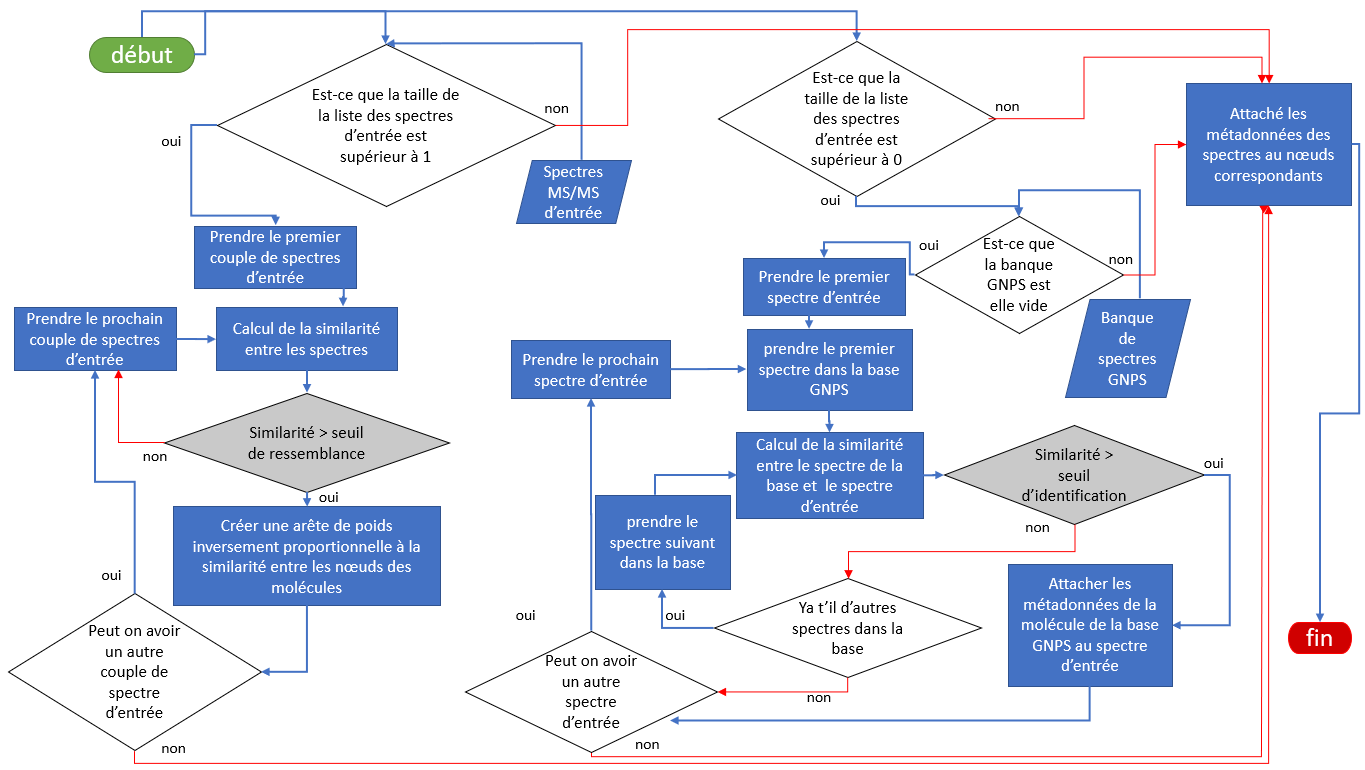
\includegraphics[width=\linewidth]{Images/organigramme_gnps.png}
                \caption{Organigramme GNPS}
                \label{fig:gnps_org}
            \end{figure}

            Après observatiob des spectres, on peut comprendre le choix de la mesure de similarité. Le cosinus de similarité permet de savoir si deux vecteurs sont colinéaires ou sont proches de l’être, ce qui le rend moins sensible aux données parses et dispersées comme les spectres de Surfacins de la figure \ref{fig:spectresmssurfacin}.

            En termes de complexité, nous pouvons aussi remarquer qu’en supposant "\textbf{T}", le nombre de spectres dans la base de données GNPS publiques et "\textbf{n}" le nombre de spectres, on aura le nombre d’opérations de calcul de similarité de la branche de calcul du graphe étant $ \frac{n \times (n-1)}{2}$, et de celui de l’identification étant égale au pire des cas à $n\times T$.

            Du workflow de GNPS, on peut remarquer qu’on fait de la déréplication de molécules, car on peut retrouver des molécules qui existent déjà (dans la base publique GNPS) sur la base de leurs spectres. Également on peut avoir des indices pour retrouver et identifier ceux qui ne se trouvent pas dans la base GNPS, par le biais des relations et des patterns communs entre ceux connus et ceux inconnus. De ce fait que peut-on dire du cas de MADByTE ?
            
    \section{MADByTE}
        L'outil MADByTE (Metabolomics And Dereplication By Two-dimensional Experiments) est une solution à la problématique attaquée par l'article \cite{egan2021development}, qui est celui de l’annotation de mixtures (mélanges) complexes de produits naturelles en utilisant la spectrométrie 2D-RMN. Pour résoudre à cette problématique, des solutions ont été créés, mais toutes n'étaient pas suffisamment simple pour caractériser l'espace chimique des spectres 2D-RMN. C’est-à-dire qu’ils n'étaient pas suffisamment simples pour avoir des résultats aisément interprétables pour l'annotation, et pour la hiérarchisation des spectres 2D-RMN dans le sens du regroupement, ce qui est utile pour la déréplication. Les spectres HSQC et TOSCY étant les spectres d’entrée du workflow de MADByTE, il est donc important de présenter ce qu’ils décrivent.

        \subsection{Spectres RMN, HSQC et TOCSY}
            Un spectre RMN est la donnée obtenue après spectroscopie par résonnance magnétique nucléaire qui consiste à exciter des atomes pouvant avoir un champ magnétique (spin), la résonnance crée par un champ magnétique spécifique. L’ensemble des déplacements chimiques de ces atomes excités sont ainsi capturés pour obtenir une donnée qui correspond au spectre RMN.
            
            En pratique on parle de spectre 1D-RMN  lorsqu’on ne s’appuie que sur les déplacements d’un type d’atomes précis, comme le proton $^{1}H$ dans le cas de l'éthonal se trouvant sur la figure \ref{fig:spectrermnethanol}. De plus on parle de spectres 2D-RMN lorsqu’on s’appuie sur les déplacements chimiques de deux types d’atomes, qui seront croisés d’une certaine manière. 

            \begin{figure}
                \centering
                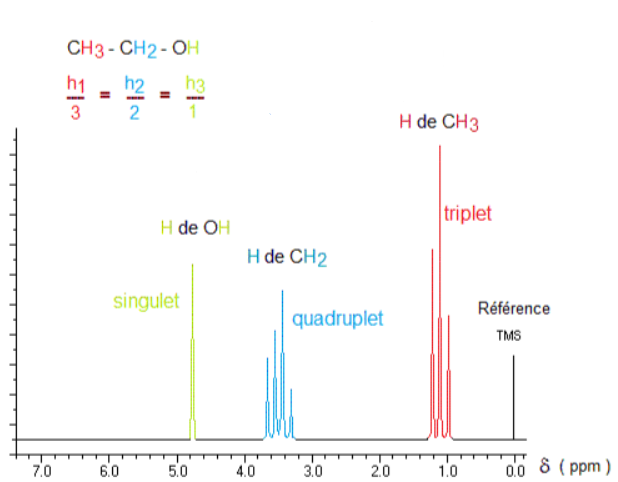
\includegraphics{Images/h-rmn-ethanol.png}
                \caption{
                Spectre RMN de l'éthanol \href{https://www.thinglink.com/scene/521604463673212930}{1}
                }
                \label{fig:spectrermnethanol}
            \end{figure}

            Prénoms l’exemple des spectres HSQC \ref{fig:spectrehsqcunknown}, on a deux types d’atomes ciblés comme le Carbonne $^{13}C$ et le proton $^{1}H$, dont les déplacements seront croisés afin de reconnaitre des liaisons directes $C-H$. Le croisement est par création de couples de déplacements chimiques en $^{13}C$ et en $^{1}H$ référant à des signaux (taches). On obtient donc ainsi une carte de taches des déplacements des deux directions $^{13}C$ et $^{1}H$, associés à leurs intensités. Pour les spectres TOCSY on fait pareil ,à la seule différence qu’on s’appuie deux fois sur les déplacements de protons $^{1}H$, ce qui conduit à chercher les protons $^{1}H$ d’environnements chimiques proches.

            \begin{figure}
                \centering
                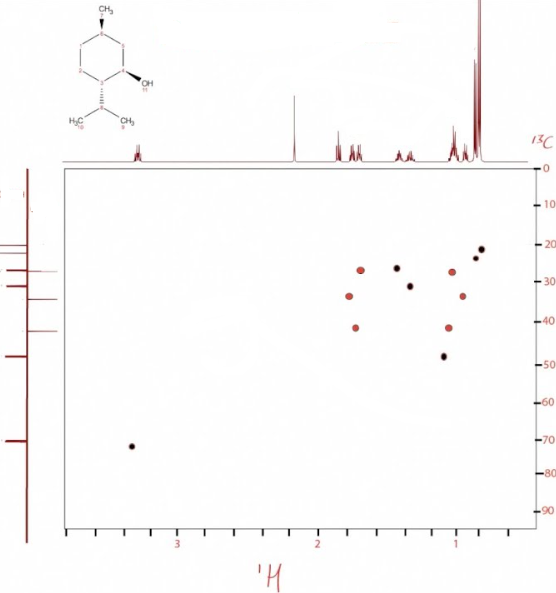
\includegraphics{Images/hsqc-unknown.png}
                \caption{
                Spectre HSQC d'une molécule inconnu \href{https://www.youtube.com/watch?v=66IvCelmABY}{2}
                }
                \label{fig:spectrehsqcunknown}
            \end{figure}
            
            On peut donc se rendre compte que, si on a connaissance des relations $C-H$ et des protons d’environnements chimiques proches (des protons associés à des carbones liées directement), on peut avoir une signature de la structure moléculaire d’une molécule. La raison pour utiliser des spectres HSQC et TOCSY est donc logique. Alors comment MADByTE les utilisent pour réaliser de la déréplication de molécules.

        \subsection{Workflow de MADByTE et déréplication}

        Sachant que la spectrométrie de masse a un inconvénient majeur, celui de dépendre de la qualité de l'ionisation, MADByTE à choisir d’utiliser les spectres RMN, HSQC et TOCSY d’entrée de molécules pour effectuer de la déréplication.

        Le workflow \ref{fig:madbyte} (à organigramme \ref{fig:madbyte_org}) s’effectue en un certain nombre d’étapes :
        \begin{figure}
            \centering
            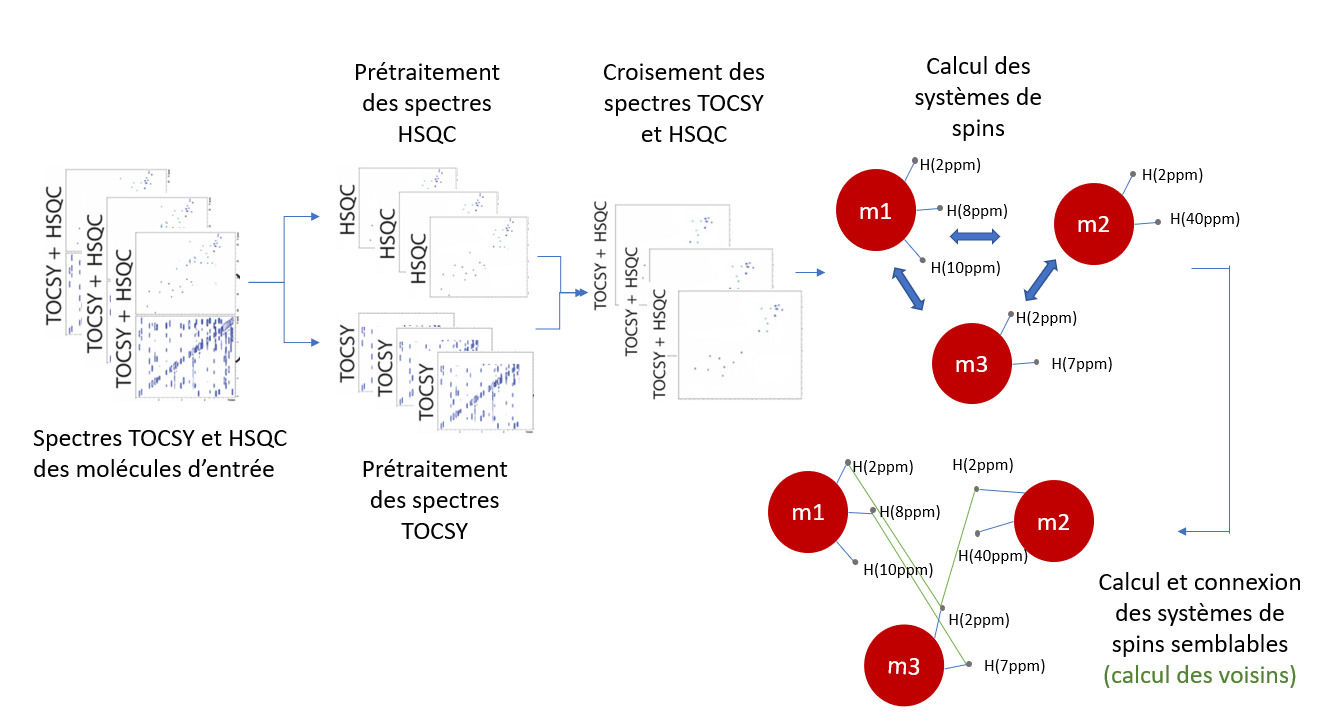
\includegraphics[width=\linewidth]{Images/madbyte.png}
            \caption{Vue simplifiée de MADByTE}
            \label{fig:madbyte}
        \end{figure}

        \begin{figure}
            \centering
            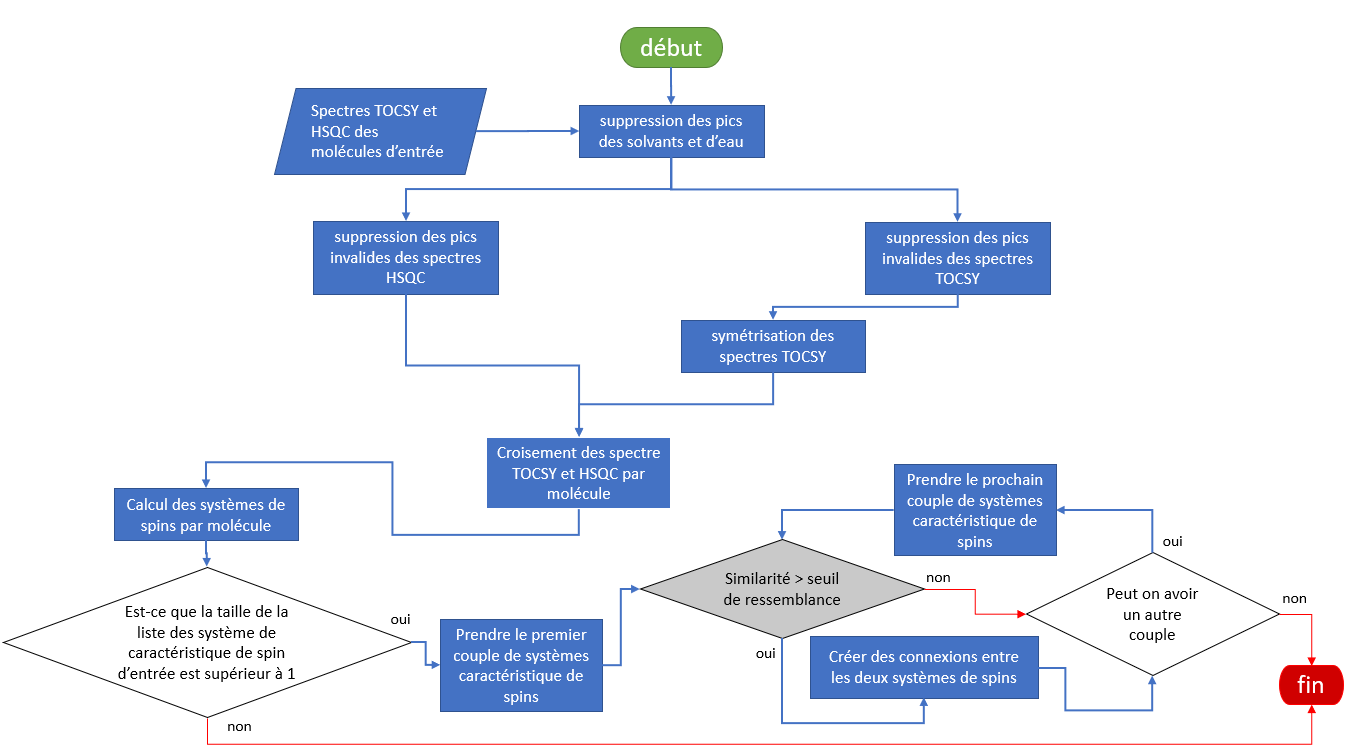
\includegraphics[width=\linewidth]{Images/organigramme_madbyte.png}
            \caption{Organigramme du workflow de MADByTE}
            \label{fig:madbyte_org}
        \end{figure}

        \begin{enumerate}
            \item Le prétraitement de chacun des spectres HSQC -TOCSY de molécules:

            Elle s’effectue parallèlement sur les spectres HSQC et TOCSY et consiste à la sélection des signaux des spectres utilisables. En ce qui concerne les spectres HSQC, les pics (ou encore signaux) invalides sont caractérisés par les déplacements chimiques sur les dimensions H et C se trouvant sur le tableau \ref{tab:hsqcinvalides}, et pour les spectres TOCSY,  les pics invalides sont ceux issus des déplacements chimiques des dimensions $^{1}H$ inférieur ou égale à \textbf{2.5 ppm}.

            \item -	Croisement de chacun des spectres HSQC -TOCSY de molécules:
            
            Elle consiste à conserver les signaux qui correspondent (suivant la dimension de proton H) entre les spectres HSQC et TOCSY

            \item Création des caractéristiques de systèmes de spins de chacun des spectres HSQC-TOCSY croisés de molécules : 

            Elle consiste à transformer chacun des spectres HSQC-TOCSY en sous graphes où pour un spectre HSQC-TOCSY, on a un nœud central caractérisant la molécule et des nœuds secondaires caractérisant les signaux contenus sur le spectre.

            \item -	 Liaison des caractéristiques de systèmes de spins semblables

            Elle consiste à lier ces dernières, en créant des liaisons entre les nœuds secondaires semblables des sous graphes semblables. Pour définir que deux caractéristiques de systèmes de spins A et B sont semblables, on calcule le score de ressemblance \ref{form:scorelikeness} et on vérifie s’il est supérieur à un seuil de ressemblance choisi. Plus ce seuil sera pétit, plus on éffectuera de l'exploration de liaisons.

        \end{enumerate}

        \begin{table}
            \centering
            \begin{tabular}{|C{2cm}|C{1cm}|}
                \hline $\ce{^{1}_{}H}$  & $\ce{^{13}_{}C}$ \\
                \hline  > 7 ppm & < 50 ppm\\
                \hline  < 7 ppm & > 170 ppm\\
                \hline  < 2.4 ppm & > 100 ppm\\
                \hline 
            \end{tabular}
            \caption{Déplacements chimiques invalides des spectres HSQC \cite{egan2021development}}
            \label{tab:hsqcinvalides}
        \end{table}

        \begin{equation}
            score(A,B) = \frac{nombre\ de\ couples (\ce{^{1}_{}H},\ce{^{13}_{}C}) \ identiques\ de\ A\ et\ de\ B}{nombre\ total\ de\ couples (\ce{^{1}_{}H},\ce{^{13}_{}C}) \ correspondantes\ de\ A\ et\ de\ B}
            \label{form:scorelikeness}
        \end{equation}

        On peut donc remarquer que si on considère avoir "\textbf{n}" spectres HSQC-TOCSY en entrée, on aura $\frac{n \times (n-1)}{2}$  calculs de score de ressemblance à effectuer.
        
        Au bout du procéssus, on obtient un réseau, qui permet de voir directement des ressemblances entre des molécules dont les spectres HSQC et TOCSY ont été passés en entrée. Il faut noter que les spectres HSQC et TOCSY de molécules permettent déjà à eux seul d’identifier des molécules qu’on qualifiera de simple (qui ne sont pas des molécules complexes). Donc certaines molécules pourront être identifié et d’autres pas manuellement, ce qui nous conduit à avoir des liaisons entre spectres connus et inconnus. MADByTE permet aussi d’après la littérature de conserver des molécules retrouvées dans sa base, afin de les introduire dans de future exécution du workflow.

        De ce constat, la déréplication de molécule s’effectue alors, en s’appuyant sur les signaux de spectres HSQC-TOCSY croisées, valides et communes entre les spectres, et qui sont visibles sur le graphe final par des liaisons entre des nœuds secondaires. Il faut noter que le seuil de ressemblance doit être donner par des experts avec soin dans le but d’avoir un bon établissement de ces liaisons.

        On peut donc à travers les workflows de GNPS et de MADByTE, comprendre que l’on cherche à identifier des molécules via des relations entre elles et des connaissances qu’on a déjà des molécules elles même. Ces connaissances sont soit contenues dans une base (cas de GNPS), soit ceux d’experts s’appuyant sur les spectres eux même (cas de MADByTE). Ces relations permettant de retrouver des patterns communs de signaux et ou encore de pics. En connaissance de ceci, comment peut on combiner les deux workflows, celui de MADByTE et de GNPS de ces outils?
    
        \section{Idée de solution et formalisation}

        Fort du constat que les spectres MS/MS et HSQC-TOCSY permettent d’avoir des signatures de la structure moléculaire d’une molécule, et que les déréplications se réalisent sur les workflows de GNPS et de MADByTE par le biais de calcul de liens entre les spectres, nous pensons que combiner les deux, revient à introduire chacun dans le calcul de ces liens. Naïvement, le calcul des liens des spectres pourrait introduire les calculs de similarités des deux approches, et la construction des graphes pourrait tout simplement avoir le même principe.
        
        "Comment associer les deux moyens de calcul de similarité entre les spectres ?" est la question à laquelle nous devons répondre si on suit la même logique. Vue qu’on n’as pas du tout d’expertise sur comment le faire, on pourrait construit une fonction de similarité qui serait capable de le faire dans le but de maximiser l’apparition des patterns communs entre les spectres qui sont voisines \ref{fig:inference}. L’entrainement de cette fonction \ref{fig:train} devra donc se faire par sa correction de constructions des voisins dans le but de maximiser la construction des patterns communs.

        \begin{figure}
            \centering
            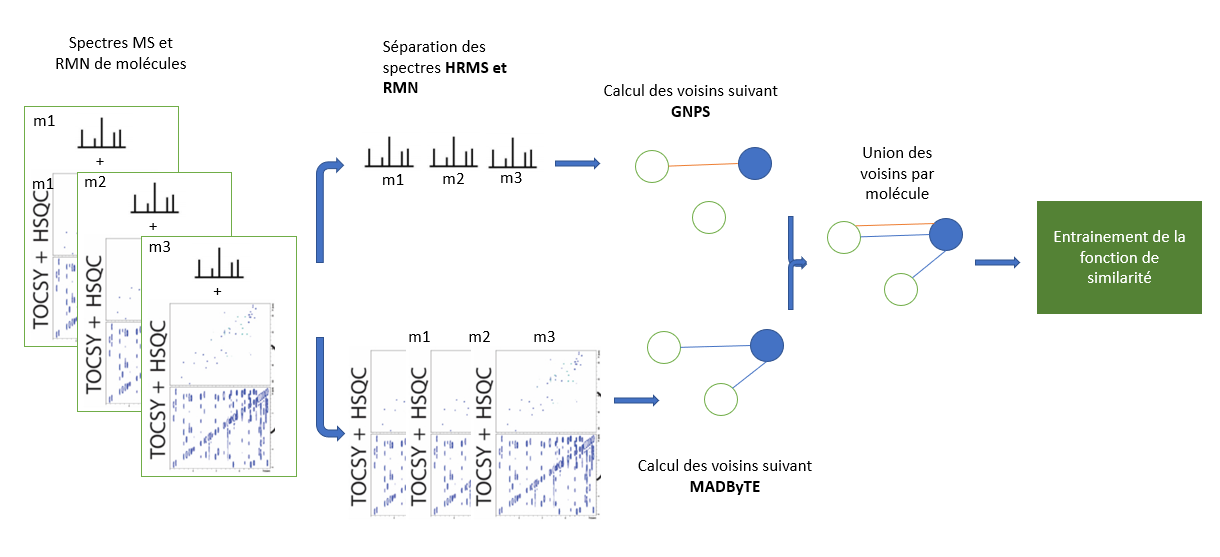
\includegraphics[width=\linewidth]{Images/idee_entrainement.png}
            \caption{Vue du processus d'entrainement}
            \label{fig:train}
        \end{figure}

        \begin{figure}
            \centering
            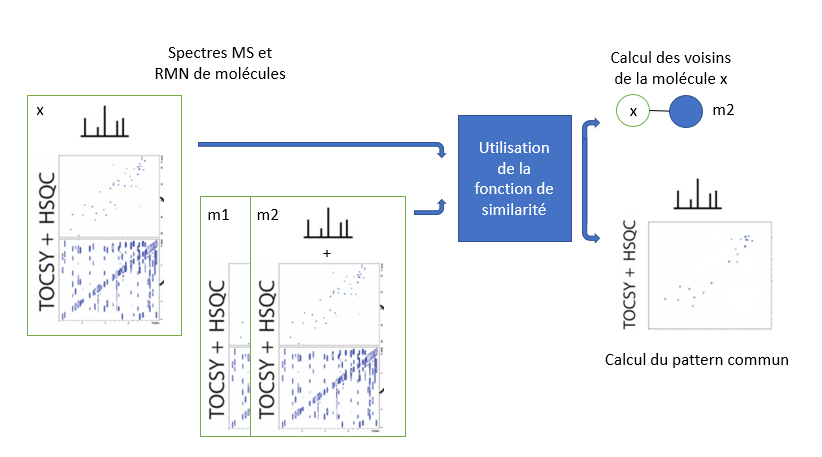
\includegraphics[width=\linewidth]{Images/idee_inference.png}
            \caption{Entrées et sorties du modèle}
            \label{fig:inference}
        \end{figure}
        
        D’où la formalisation suivante :

        Soient $M =\{ {m_{1}},{m_{2}}...,{m_{n}} \}$ (où $m_{i} = (ms_{i}, rmn_{i})$) l'ensemble des molécules connues, $sim$ la fonction de similarité a utilisée qui décrit la probabilité que deux molécules soient semblables, $e = (e_{ms}, e_{rmn})$ le couple de seuil utilisé pour les processus simplifiés de GNPS et de MADByTE, 
        l'ensemble des molécules voisines $\eta(x,e)$ de $x$ par rapport au seuil $e$ calculé en utilisant les étapes dédiées de GNPS et de MADByTE et $patternCommun$ la fonction permettant de calculer les paterns communs d'un ensemble de molécules.
        
        Pour chacune des molécules $x$ de $M$, le pattern commun $\tilde{x}$ entre les molécules voisines $\eta(x,e)$ et $x$ est définier sur la formule \ref{form:pattern}
        
        \begin{equation}
            \tilde{x} = patternCommun( \{x\} \cup \eta(x,e))
            \label{form:pattern}
        \end{equation}
        
        On souhaite que $\tilde{x}$ soit similaire le plus possible à toutes les molécules voisines et $\eta(x)$ et à $x$. Ce qui conduit à la maximisation de la fonction $f$ suivante:
        \begin{equation}
             f(x, e, sim) =  \frac{1}{|\eta(x,e)|} \times \sum_{ m \in \eta(x,e) } sim(\tilde{x}, m)
        \end{equation}
        \begin{equation}
            \eta(x,e)= \eta'(x) \cup \{voisins\ de\ x\ selon\ GNPS\ et\ MADByTE\}
        \end{equation}
        \begin{equation}
            \eta'(x) = \{ m_{i} | m_{i} \in M , sim(x, m_{i}) > 0.5 \}
        \end{equation}
        
        Dans le but d'utliser les mesures de similarité, nous proposons la fonction $sim$ suivante, pour calculer pour un molécule x de M l'ensemble de ces voisins $\eta'(x)$
        \begin{equation}
            sim(x1,x2)= y(\alpha,x1 ,x2) =  sigmoid( \alpha_{1}\times\cos(ms_{x1}, ms_{x2}) + \alpha_{2}\times{score(rmn_{x1}, rmn_{x2})} )
        \end{equation}

        La fonction pourra ainsi etre apprise selon les valeurs de seuil de similarité de GNPS et MADByTE pour réaliser de la déréplication en faisant de l'exploration ou non.
        
        
        \section{Conclusion}
            En définitive, nous avons parlé de la déréplication, plus précisément de sa fonction et du pourquoi il permettait d'identifier une molécule dit inconnu, et présenté une idée de combinaison qui permettrait de combiner l'utilisation des données $MS$ et $HSQC$-$TOCSY$ pour l'identification de molécule en s'appuyant sur des procéssus simplifié de GNPS et de MADByTE. Cette approche proposé s'appuie sur l'hypothèse, l'identification une molécule inconnu est un ensemble de pics et de déplacements communs entre les spectres de molécules(qui est un paramètre important qui n'as pas été explicitement défini), mais ne prend pas en compte les seuils à partir duquel on considère que deux molécules sont identiques mais uniquement le seuil à partir duquel deux molécules sont semblables. Comment le prendre en compte, pourrais être l'objet d'une autre analyse.

\bibliographystyle{plain}
    \bibliography{reference_GNPS_MADByTE}
    
\end{document}